\section{Data and empirical designs}\label{app:data}

All scripts are in \texttt{empirics/} and run in numerical order. Raw data are
public.

\paragraph{The arXiv panel.} The source is the arXiv metadata snapshot
distributed by Cornell University on Kaggle, file dated 18 October 2026
\citep{kaggle2026}. We keep the 2,214,380 papers with new-style identifiers from
January 2015 (\texttt{01\_parse\_snapshot.py}). For each paper we record the
submitter's name, the parsed author list, the categories (the first is the
primary category), title, abstract, and the timestamp of version 1, which is
the submission time in UTC. The last submission in the snapshot was made at
13:59:59 ET on 15 October 2026, just before that day's cutoff.

\paragraph{Announcement batches and listing position}
(\texttt{02\_listing\_position.py}). Each paper is assigned the deadline it was
submitted against: the same weekday's cutoff if submitted before it, otherwise
the next weekday's. Weekend submissions belong to Monday's batch. The cutoff was
16:00 ET until 30 December 2016 and 14:00 ET from 2 January 2017. Both are
visible as spikes in the distribution of submission times. Identifiers are
assigned at announcement, so the smallest identifier among the papers with a
given deadline marks the start of that announcement block. Every paper is
placed in the block its identifier falls in. Papers placed in a later block than
their deadline were held for moderation (6.1\%). Within blocks, the rank
correlation between identifier and submission time is 0.98 for papers not held
(median over 3,065 blocks). Position is the rank by identifier within block and
primary category. Block starts are monotone except at seven holiday periods,
which we drop: 17 December to 8 January and the week of US Thanksgiving.

\paragraph{Cutoff design} (\texttt{03\_rd\_sample.py}, \texttt{07\_rd.py}).
Weekday submissions within 180 minutes of the cutoff, deadlines from 9 January
2017 to 16 December 2022 (272,707 papers). The running variable is minutes from
the cutoff. Estimates are local linear with separate slopes, a triangular
kernel, category-year and weekday fixed effects, and standard errors clustered
by submission day. The density of the running variable is discontinuous by
construction, since authors bunch in the first seconds after the cutoff, so the
main specification uses a donut of five minutes. Results for bandwidths of 30,
60, 120 and 180 minutes and donuts of 0, 5 and 10 minutes are in
\texttt{empirics/results/rd.json}.

\paragraph{Rank design} (\texttt{09\_hep\_sample.py}, \texttt{10\_hep\_pairs.py},
\texttt{11\_rank\_design.py}). All papers with primary category hep-th, hep-ph,
hep-ex, hep-lat, gr-qc, nucl-th, nucl-ex, astro-ph.CO or astro-ph.HE, announced
in their regular batch, 2017--2022, outside holidays (101,392 papers; 87,694
submitted at least 15 minutes after the batch opened). The time since the batch
opened is measured from the previous weekday's 14:00 ET cutoff.

\paragraph{Overlap measures} (\texttt{neardup.py}). Within each primary category,
papers from July 2016 to December 2024 are represented by TF-IDF vectors of title
and abstract: sublinear term frequencies, English stop words removed, terms in at
least two and at most 30\% of the category's papers. For a random sample of
3,000 papers from 2018 on, we compute the cosine similarity to the nearest
earlier paper in the category within 24 months. Its percentiles define the
category's thresholds $\tau_q$. For each focal paper we keep every later paper in
the category within 730 days whose similarity is at least $\tau_{50}$. A pair is
a \emph{self} pair if the two author lists share a name key. Half of all pairs at
$\tau_{50}$ are self pairs, and at $\tau_{95}$ the share is 87\%, which is why
the overlap outcomes use lower thresholds than the descriptive flag.

\paragraph{Citations and references.} INSPIRE-HEP's public API gives citation
counts excluding self-citations and curated reference lists, linked by record
identifiers (\texttt{inspire\_fetch.py}). Coverage of the high-energy-physics
sample is above 99.9\%. For other fields we use the Semantic Scholar batch API
(\texttt{s2\_fetch.py}), whose reference lists are often withheld for arXiv
papers (41\% coverage among later overlapping papers). The cutoff design
therefore reports all-field citations for the subsample fetched by the time of
writing.

\paragraph{Name keys} (\texttt{names.py}). Names are transliterated to ASCII, TeX
accents removed, and keyed as first name plus last name for submitters and as
first initial plus last name for authors (full first names where the parsed
author list has them, for the rotation analysis). Name keys are used instead of
database author identifiers, which were reissued for many authors in 2025. Shared
names produce collisions. The designs either difference them out (endorsement,
LLM adoption) or remove them explicitly (submission cap: names whose submissions
in a half-month span several archives).

\paragraph{Endorsement} (\texttt{06\_entry\_policies.py}). A paper has a
first-time submitter if the submitter's name key has not submitted since 2015.
It has a submitter with no prior authorship if, in addition, the submitter's
initial key appears in no earlier author list. Weekly cells by announcement week
and group (Mathematics, other sections), September 2024 to October 2026. Each
week of the 2025--26 academic year is differenced against the same week of
2024--25.

\paragraph{CS review policy} (\texttt{06\_entry\_policies.py}). A title is
review-type if it contains survey, review, overview, tutorial, position paper,
``position:'', primer, roadmap, perspective, state of the art or systematic
literature. The dose-response uses the 29 computer-science categories with at
least 300 papers in each Nov--Oct year from 2023--24 to 2025--26. A paper has a
first-time author if any author with a full first name has a key never seen
before.

\paragraph{Submission cap} (\texttt{05\_cap.py}). Days 1--15 of each month,
papers announced in their regular batch. A submission is excess if it is the
submitter's third or later in the half-month, and clean if all of the name's
submissions in that half-month fall in one archive and the submitter is not a
proceedings account.

\paragraph{LLM-style writing} (\texttt{08\_llm\_authors.py}). Marker words:
delve, showcase, underscore (all inflections), intricate, intricacies, meticulous,
pivotal, realm, notably, commendable, garner, multifaceted, seamless, invaluable,
groundbreaking, tapestry, elucidate. Their share of abstracts was 2.1\% in 2019,
3.0\% in 2022, 10.6\% in 2024 and 4.4\% in 2026. The decline in 2026 suggests that
authors learned to avoid them, and it is one reason to classify adoption early.

\begin{figure}[t]
\centering
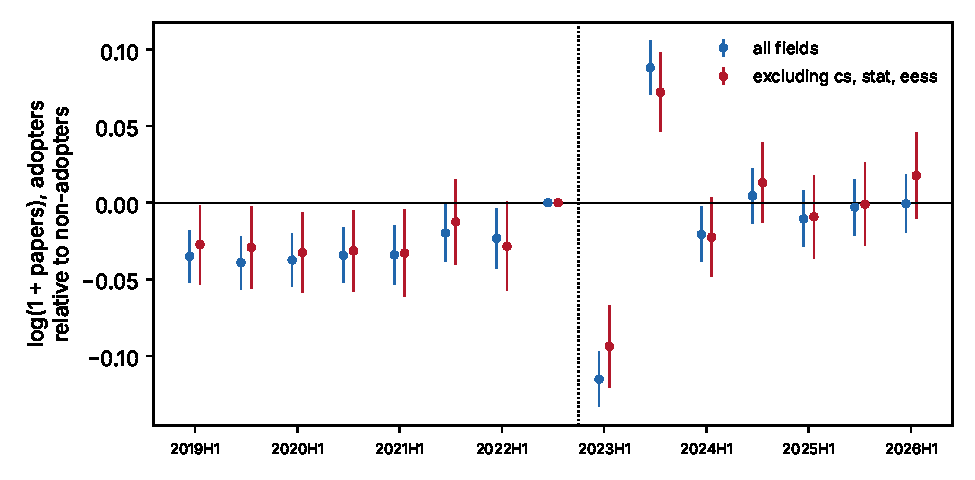
\includegraphics[width=0.75\textwidth]{figures/emp_llm_authors.pdf}
\caption{Author-level output of adopters of LLM-style writing, relative to
non-adopters (event study, reference 2022H2; 95\% intervals). Adoption is
classified from 2023 abstracts. Blue: all fields; red: excluding cs, stat and
eess.}
\label{fig:llm}
\end{figure}

\begin{figure}[t]
\centering
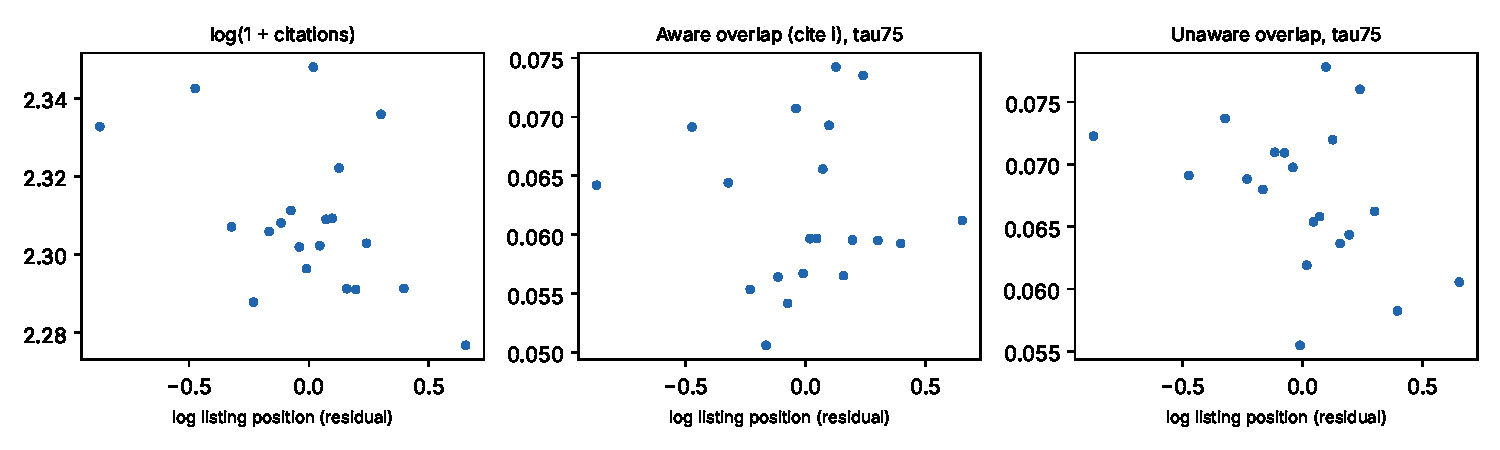
\includegraphics[width=\textwidth]{figures/emp_rank_design.pdf}
\caption{Listing rank in high-energy physics: binned residuals of outcomes on
residual log listing position (twenty bins), net of category-year and
submission-time fixed effects and log list size.}
\label{fig:rank}
\end{figure}
